% This file was created by tikzplotlib v0.9.1.
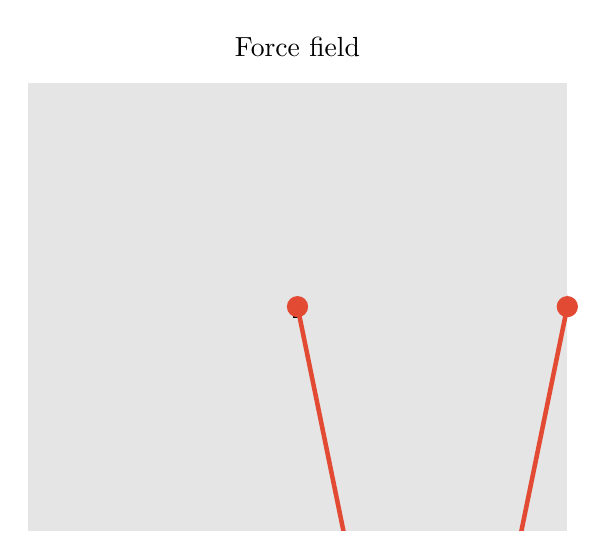
\begin{tikzpicture}

\definecolor{color0}{rgb}{0.886274509803922,0.290196078431373,0.2}

\begin{axis}[
axis background/.style={fill=white!89.8039215686275!black},
axis line style={white},
hide x axis,
hide y axis,
tick align=outside,
tick pos=left,
title={Force field},
x grid style={white},
xmajorgrids,
xmin=-0.5, xmax=0.5,
xtick style={color=white!33.3333333333333!black},
y dir=reverse,
y grid style={white},
ymajorgrids,
ymin=-0.5, ymax=0.5,
ytick style={color=white!33.3333333333333!black}
]
\draw[-latex,draw=black] (axis cs:0,0) -- (axis cs:0,0);
\draw[-latex,draw=black] (axis cs:0,0) -- (axis cs:0,0);
\draw[-latex,draw=black] (axis cs:0,0) -- (axis cs:0,0);
\draw[-latex,draw=black] (axis cs:0,0) -- (axis cs:0,0);
\draw[-latex,draw=black] (axis cs:0,0) -- (axis cs:0,0);
\draw[-latex,draw=black] (axis cs:0,0) -- (axis cs:0,0);
\draw[-latex,draw=black] (axis cs:0,0) -- (axis cs:0,0);
\draw[-latex,draw=black] (axis cs:0,0) -- (axis cs:0,0);
\draw[-latex,draw=black] (axis cs:0,0) -- (axis cs:0,0);
\draw[-latex,draw=black] (axis cs:0,0) -- (axis cs:0,0);
\draw[-latex,draw=black] (axis cs:0,0) -- (axis cs:0,0);
\draw[-latex,draw=black] (axis cs:0,0) -- (axis cs:0,0);
\draw[-latex,draw=black] (axis cs:0,0) -- (axis cs:0,0);
\draw[-latex,draw=black] (axis cs:0,0) -- (axis cs:0,0);
\draw[-latex,draw=black] (axis cs:0,0) -- (axis cs:0,0);
\draw[-latex,draw=black] (axis cs:0,0) -- (axis cs:0,0);
\draw[-latex,draw=black] (axis cs:0,0) -- (axis cs:0,0);
\draw[-latex,draw=black] (axis cs:0,0) -- (axis cs:0,0);
\draw[-latex,draw=black] (axis cs:0,0) -- (axis cs:0,0);
\draw[-latex,draw=black] (axis cs:0,0) -- (axis cs:0,0);
\draw[-latex,draw=black] (axis cs:0,0) -- (axis cs:0,0);
\draw[-latex,draw=black] (axis cs:0,0) -- (axis cs:0,0);
\draw[-latex,draw=black] (axis cs:0,0) -- (axis cs:0,0);
\draw[-latex,draw=black] (axis cs:0,0) -- (axis cs:0,0);
\draw[-latex,draw=black] (axis cs:0,0) -- (axis cs:0,0);
\draw[-latex,draw=black] (axis cs:0,0) -- (axis cs:0,0);
\draw[-latex,draw=black] (axis cs:0,0) -- (axis cs:0,0);
\draw[-latex,draw=black] (axis cs:0,0) -- (axis cs:0,0);
\draw[-latex,draw=black] (axis cs:0,0) -- (axis cs:0,0);
\draw[-latex,draw=black] (axis cs:0,0) -- (axis cs:0,0);
\draw[-latex,draw=black] (axis cs:0,0) -- (axis cs:0,0);
\draw[-latex,draw=black] (axis cs:0,0) -- (axis cs:0,0);
\draw[-latex,draw=black] (axis cs:0,0) -- (axis cs:0,0);
\draw[-latex,draw=black] (axis cs:0,0) -- (axis cs:0,0);
\draw[-latex,draw=black] (axis cs:0,0) -- (axis cs:0,0);
\draw[-latex,draw=black] (axis cs:0,0) -- (axis cs:0,0);
\draw[-latex,draw=black] (axis cs:0,0) -- (axis cs:0,0);
\draw[-latex,draw=black] (axis cs:0,0) -- (axis cs:0,0);
\draw[-latex,draw=black] (axis cs:0,0) -- (axis cs:0,0);
\draw[-latex,draw=black] (axis cs:0,0) -- (axis cs:0,0);
\draw[-latex,draw=black] (axis cs:0,0) -- (axis cs:0,0);
\draw[-latex,draw=black] (axis cs:0,0) -- (axis cs:0,0);
\draw[-latex,draw=black] (axis cs:0,0) -- (axis cs:0,0);
\draw[-latex,draw=black] (axis cs:0,0) -- (axis cs:0,0);
\draw[-latex,draw=black] (axis cs:0,0) -- (axis cs:0,0);
\draw[-latex,draw=black] (axis cs:0,0) -- (axis cs:0,0);
\draw[-latex,draw=black] (axis cs:0,0) -- (axis cs:0,0);
\draw[-latex,draw=black] (axis cs:0,0) -- (axis cs:0,0);
\draw[-latex,draw=black] (axis cs:0,0) -- (axis cs:0,0);
\draw[-latex,draw=black] (axis cs:0,0) -- (axis cs:0,0);
\draw[-latex,draw=black] (axis cs:0,0) -- (axis cs:0,0);
\draw[-latex,draw=black] (axis cs:0,0) -- (axis cs:0,0);
\draw[-latex,draw=black] (axis cs:0,0) -- (axis cs:0,0);
\draw[-latex,draw=black] (axis cs:0,0) -- (axis cs:0,0);
\draw[-latex,draw=black] (axis cs:0,0) -- (axis cs:0,0);
\draw[-latex,draw=black] (axis cs:0,0) -- (axis cs:0,0);
\draw[-latex,draw=black] (axis cs:0,0) -- (axis cs:0,0);
\draw[-latex,draw=black] (axis cs:0,0) -- (axis cs:0,0);
\draw[-latex,draw=black] (axis cs:0,0) -- (axis cs:0,0);
\draw[-latex,draw=black] (axis cs:0,0) -- (axis cs:0,0);
\draw[-latex,draw=black] (axis cs:0,0) -- (axis cs:0,0);
\draw[-latex,draw=black] (axis cs:0,0) -- (axis cs:0,0);
\draw[-latex,draw=black] (axis cs:0,0) -- (axis cs:0,0);
\draw[-latex,draw=black] (axis cs:0,0) -- (axis cs:0,0);
\draw[-latex,draw=black] (axis cs:0,0) -- (axis cs:0,0);
\draw[-latex,draw=black] (axis cs:0,0) -- (axis cs:0,0);
\draw[-latex,draw=black] (axis cs:0,0) -- (axis cs:0,0);
\draw[-latex,draw=black] (axis cs:0,0) -- (axis cs:0,0);
\draw[-latex,draw=black] (axis cs:0,0) -- (axis cs:0,0);
\draw[-latex,draw=black] (axis cs:0,0) -- (axis cs:0,0);
\draw[-latex,draw=black] (axis cs:0,0) -- (axis cs:0,0);
\draw[-latex,draw=black] (axis cs:0,0) -- (axis cs:0,0);
\draw[-latex,draw=black] (axis cs:0,0) -- (axis cs:0,0);
\draw[-latex,draw=black] (axis cs:0,0) -- (axis cs:0,0);
\draw[-latex,draw=black] (axis cs:0,0) -- (axis cs:0,0);
\draw[-latex,draw=black] (axis cs:0,0) -- (axis cs:0,0);
\draw[-latex,draw=black] (axis cs:0,0) -- (axis cs:0,0);
\draw[-latex,draw=black] (axis cs:0,0) -- (axis cs:0,0);
\draw[-latex,draw=black] (axis cs:0,0) -- (axis cs:0,0);
\draw[-latex,draw=black] (axis cs:0,0) -- (axis cs:0,0);
\draw[-latex,draw=black] (axis cs:0,0) -- (axis cs:0,0);
\draw[-latex,draw=black] (axis cs:0,0) -- (axis cs:0,0);
\draw[-latex,draw=black] (axis cs:0,0) -- (axis cs:0,0);
\draw[-latex,draw=black] (axis cs:0,0) -- (axis cs:0,0);
\draw[-latex,draw=black] (axis cs:0,0) -- (axis cs:0,0);
\draw[-latex,draw=black] (axis cs:0,0) -- (axis cs:0,0);
\draw[-latex,draw=black] (axis cs:0,0) -- (axis cs:0,0);
\draw[-latex,draw=black] (axis cs:0,0) -- (axis cs:0,0);
\draw[-latex,draw=black] (axis cs:0,0) -- (axis cs:0,0);
\draw[-latex,draw=black] (axis cs:0,0) -- (axis cs:0,0);
\draw[-latex,draw=black] (axis cs:0,0) -- (axis cs:0,0);
\draw[-latex,draw=black] (axis cs:0,0) -- (axis cs:0,0);
\draw[-latex,draw=black] (axis cs:0,0) -- (axis cs:0,0);
\draw[-latex,draw=black] (axis cs:0,0) -- (axis cs:0,0);
\draw[-latex,draw=black] (axis cs:0,0) -- (axis cs:0,0);
\draw[-latex,draw=black] (axis cs:0,0) -- (axis cs:0,0);
\draw[-latex,draw=black] (axis cs:0,0) -- (axis cs:0,0);
\draw[-latex,draw=black] (axis cs:0,0) -- (axis cs:0,0);
\draw[-latex,draw=black] (axis cs:0,0) -- (axis cs:0,0);
\draw[-latex,draw=black] (axis cs:0,0) -- (axis cs:0,0);
\draw[-latex,draw=black] (axis cs:0,0) -- (axis cs:0,0);
\draw[-latex,draw=black] (axis cs:0,0) -- (axis cs:0,0);
\draw[-latex,draw=black] (axis cs:0,0) -- (axis cs:0,0);
\draw[-latex,draw=black] (axis cs:0,0) -- (axis cs:0,0);
\draw[-latex,draw=black] (axis cs:0,0) -- (axis cs:0,0);
\draw[-latex,draw=black] (axis cs:0,0) -- (axis cs:0,0);
\draw[-latex,draw=black] (axis cs:0,0) -- (axis cs:0,0);
\draw[-latex,draw=black] (axis cs:0,0) -- (axis cs:0,0);
\draw[-latex,draw=black] (axis cs:0,0) -- (axis cs:0,0);
\draw[-latex,draw=black] (axis cs:0,0) -- (axis cs:0,0);
\draw[-latex,draw=black] (axis cs:0,0) -- (axis cs:0,0);
\draw[-latex,draw=black] (axis cs:0,0) -- (axis cs:0,0);
\draw[-latex,draw=black] (axis cs:0,0) -- (axis cs:0,0);
\draw[-latex,draw=black] (axis cs:0,0) -- (axis cs:0,0);
\draw[-latex,draw=black] (axis cs:0,0) -- (axis cs:0,0);
\draw[-latex,draw=black] (axis cs:0,0) -- (axis cs:0,0);
\draw[-latex,draw=black] (axis cs:0,0) -- (axis cs:0,0);
\draw[-latex,draw=black] (axis cs:0,0) -- (axis cs:0,0);
\draw[-latex,draw=black] (axis cs:0,0) -- (axis cs:0,0);
\draw[-latex,draw=black] (axis cs:0,0) -- (axis cs:0,0);
\draw[-latex,draw=black] (axis cs:0,0) -- (axis cs:0,0);
\draw[-latex,draw=black] (axis cs:0,0) -- (axis cs:0,0);
\draw[-latex,draw=black] (axis cs:0,0) -- (axis cs:0,0);
\draw[-latex,draw=black] (axis cs:0,0) -- (axis cs:0,0);
\draw[-latex,draw=black] (axis cs:0,0) -- (axis cs:0,0);
\addplot [line width=1.64pt, color0, mark=*, mark size=3, mark options={solid}]
table {%
0 0
0.1 0.587785252292473
0.2 0.951056516295154
0.3 0.951056516295154
0.4 0.587785252292473
0.5 1.22464679914735e-16
0.6 -0.587785252292473
0.7 -0.951056516295154
0.8 -0.951056516295154
0.9 -0.587785252292473
1 -2.44929359829471e-16
1.1 0.587785252292474
1.2 0.951056516295154
1.3 0.951056516295154
1.4 0.587785252292473
1.5 3.67394039744206e-16
1.6 -0.587785252292473
1.7 -0.951056516295154
1.8 -0.951056516295154
1.9 -0.587785252292473
};
\end{axis}

\end{tikzpicture}
